\documentclass[
               12pt,             %Tamanho da fonte
               a4paper,          % Tamanho do papel em que será impresso
               chapter=TITLE,    % títulos de capítulos convertidos em letras maiúsculas
               section=TITLE,    % títulos de seções convertidos em letras maiúsculas
               english,
               brazil            
]{article}

\usepackage[brazil]{babel}
\usepackage[utf8]{inputenc}
\usepackage[normalem]{ulem}
\usepackage[T1]{fontenc}
\usepackage{lipsum}
\usepackage{cmap}
\usepackage{xcolor}
\usepackage{graphicx}
\usepackage[brazilian,hyperpageref]{backref}
\usepackage[alf]{abntex2cite}
\usepackage{indentfirst} %Para gerar o espaçamento de paragrafo no inicio das linhas
\usepackage{setspace} %Espaçamento entre linhas
\usepackage[top=3cm, bottom=2cm, left=3cm, right=2cm]{geometry} %Setando manualmente o espaçamento de margem da folha
\usepackage[pdftex]{hyperref} %Geração de links 
\usepackage{listings} %Colocação de codigo fonte, no caso shellscript

\definecolor{verde}{rgb}{0,0.5,0}
\definecolor{jpurple}{rgb}{0.5,0,0.35}
\definecolor{verde}{rgb}{0.25,0.5,0.35}
\definecolor{verde}{rgb}{0,0.5,0}


\lstset{
  language=C,
  basicstyle=\ttfamily\small, 
  keywordstyle=\color{blue}, 
  stringstyle=\color{verde}, 
  commentstyle=\color{red}, 
  extendedchars=true, 
  showspaces=false, 
  showstringspaces=false, 
  numbers=left,
  numberstyle=\tiny,
  breaklines=true, 
  backgroundcolor=\color{green!10},
  breakautoindent=true, 
  captionpos=b,
  xleftmargin=0pt,
}





\begin{document}

\pagestyle{empty} %Removendo paginação do documento.

%%%%%%%%%%%%%%%%%%%%%%%%%%%%%%%%%%%%%%%%%%%%%%%%%%%%%%%%%%%%%%%%%%%%%%%%%%%%%%%%%%%%%%%%%%%%%%%%%%%%%%%%%%%%%%%%%%%%%%
% capa

\begin{titlepage} 									%Inicio capa

	\begin{center} 									%Topo da pagina
		{\large Willian Mendonça}\\[0.2cm] 			%0,2cm é a distância entre as linhas de texto
		{\large Analista de Redes}\\[5.3cm]
	\end{center} 									%Fim topo
	
	\begin{center} 									%inicia o trecho do texto que vai no meio da pagina
		{\bf \huge Instalação e configuração}\\[0.2cm]
		{\bf \huge Servidor OCS}\\[13cm] 			% \bf = negrito  \huge = texto enorme
	\end{center} 									%términa o trecho do texto que vai no meio da pagina
	
	\begin{center} 									%Radapé da pagina
		{\large São José dos Campos}\\[0.2cm]
		{\large 2017}
	\end{center} 									%Fim rodapé
	
\end{titlepage} 									%Fim capa

\pagebreak 											%Quebra de pagina

													%Fim capa
%%%%%%%%%%%%%%%%%%%%%%%%%%%%%%%%%%%%%%%%%%%%%%%%%%%%%%%%%%%%%%%%%%%%%%%%%%%%%%%%%%%%%%%%%%%%%%%%%%%%%%%%%%%%%%%%%%%%%%

\setstretch{1.5} %Setando o valor do espaçamento

\section{Introdução}

O OCS inventory NG (\textit{Open Computer and Software Inventory Next Generation}) é um \textit{software} livre que permite aos administradores de rede gerar um inventario completo de seus ativos de TI. O OCS-NG coleta informações sobre o  \textit{software} e o \textit{hardware} das maquinas em rede que executam seu agente ("\textit{OCS inventory agent}"). As informações coletadas são organizadas e gravadas em um banco de dados instalado no servidor, o OCS utiliza uma interface \textit{WEB} pra exibir ao usuário ou administrador de rede as informações coletadas de forma amigável. O OCS também conta com uma função chamada \textit{IpDiscover} que funciona como um SNMP \textit{scan} que identifica todos os equipamentos da rede.\\

O principio de funcionamento do OCS é o seguinte, o agente se comunica com o servidor (nunca o contrario) e envia as informações de inventario em formato XML essa informações são tratadas pelo servidor e gravadas no banco de dados MySQL. As trocas de informações entre cliente e servidor podem ser feitas via HTTP ou HTTPS, as transmissões de \textit{software} e SNMP \textit{scan} são feitos somente em HTTPS.\\

O servidor de gerenciamento do OCS-NG é composto basicamente por quatro elementos, são eles: Servidor de banco de dados, que armazena informações de inventário (MySQL), servidor de comunicação, que lida com as comunicações HTTP ou HTTPs entre o servidor de banco de dados e agentes (Apache e Perl), console de administração, que permite aos administradores consultar o servidor de banco de dados usando seu navegador favorito (Apache, php) e o servidor de implantação, que armazena toda a configuração de implementação do pacote (Apache, ssl).

\pagebreak

\section{Instalação}

\subsection{Sistema Operacional}

Nesse documento, o OCS-NG será instalado no Debian 8 (Jessie) amd64. O Debian foi escolhido devido a sua estabilidade e também a constante atualização do sistema operacional, claro que a facilidade de suporte e de utilização do sistema também foram pontos extremamente relevantes para sua escolha como base para esse projeto. O Debian tem um excelente desempenho mesmo com inúmeras adversidades e funciona extremamente bem em qualquer circunstância.\\

A instalação do sistema operacional, nesse caso, não contou com nenhum passo fora do comum, a mesma não será abordada com profundidade visto que não é o foco deste documento, foram criadas 3 partições (\textit{Home}, \textit{SWAP} e $\backslash$\footnote{Partição raiz do sistema operacional, equivalente ao disco C do Windows}) durante a instalação foi utilizado um espelho de rede para configurar o apt e também para manter o sistema atualizado desde a instalação, o espelho utilizado foi "ftp.br.debian.org".\\

Foi finalizada a instalação utilizando somente as opções \textit{standard} do sistema operacional,sem nenhum pacote adicional até o momento. Todas as instalações necessárias serão feitas no momento em que as mesmas forem solicitadas, lembrando que esse servidor está sendo montado única e exclusivamente para o uso do OCS-NG, ou seja, inventario será a única função desse servidor.\\


\subsection{OCS-NG}

\subsubsection{Preparação}

Antes de iniciar os procedimentos de instalação é necessário que alguns ajustes sejam feitos no servidor, (estamos considerando um servidor que acabou de ser instalado):\\

\pagebreak

\begin{itemize}

\item Setar IP fixo no servidor, para que o Agente sempre saiba com quem se comunicar, o procedimento será realizado da seguinte forma:\\
		Edite o arquivo \textit{interfaces}:
		
		\begin{verbatim}
			nano /etc/network/interfaces
		\end{verbatim}		 

		E substitua:
		
		\begin{verbatim}
			The primary network interface
			allow-hotplug eth0
			iface eth0 inet dhcp
		\end{verbatim}		 
		
		Por: 
		
		\begin{verbatim}
			auto eth0
			iface eth0 inet static
			address 192.168.XXX.XXX
			netmask 255.255.XXX.XXX
			gateway 192.168.XXX.XXX
		\end{verbatim}	

		Claramente, colocando informações reais da sua rede local.
		

\item Alterar o arquivo sources.list para ignorar o cd de instalação na busca por pacotes, basta editar o aqruivo com o comando: 

		\begin{verbatim}
			nano /etc/apt/sources.list
		\end{verbatim}	

E comentar, utilizando o carácter \# no inicio das linhas que comecem com "deb cdrom:" sem aspas.

		
\end{itemize}

Preparações finalizadas, vamos prosseguir com a instalação.

\subsubsection{Instalação}

A instalação do OCS-NG pode ser feita utilizando seu código fonte, disponível em \href{www.ocsinventory-ng.org}{www.ocsinventory-ng.org} junto com a documentação oficial do produto. Nesse documento faremos o download do código fonte e compilaremos o mesmo. A instalação se inicia com os seguintes passos, segia os comandos:

OBS: ABSOLUTAMENTE TODOS OS COMANDOS DESSE DOCUMENTO PRECISAM SER EXECUTADOS COMO root.

\begin{lstlisting}
# apt update && apt upgrade
# apt install apt-build vim
# apt install apache2 libmysqlclient15-dev mysql-server php5 php5-gd php5-mysql php5-curl php5-imap php5-ldap
/* ATENCAO Nesse momento sera solicitado a senha do MySQL-Server */
# apt install libapache-dbi-perl libnet-ip-perl libsoap-lite-perl libapache2-mod-perl2 libxml-simple-perl libcompress-zlib-perl libdbi-perl libdbd-mysql-perl
/* Os modulos do CPAN precisam ser instalados manualmente */
# perl -e shell -MCPAN
  CPAN*> install CPAN
  CPAN*> reload CPAN
  CPAN*> install XML::Entities
  CAPN*> exit
/* Reinicie o servico do APACHE para que as confgs entrem em vigor */
# /etc/init.d/apache2 restart
\end{lstlisting} 

Nesse momento, temos um ambiente preparado para receber o OCS-NG com servidor \textit{WEB} (\textit{Apache}) e também o servidor de banco de dados (\textit{MySQL}), sendo assim, podemos prosseguir para a instalação do OCS-NG propriamente dita, será feito \textit{download}, compilação e instalação do OCS-NG passo a passo.\\

\begin{lstlisting}
/* Pasta escolhida para download /opt */
# cd /opt
# wget https://github.com/OCSInventory-NG/OCSInventory-ocsreports/releases/download/2.3.1/OCSNG_UNIX_SERVER-2.3.1.tar.gz
# tar -xzvf OCSNG_UNIX_SERVER-2.3.1.tar.gz
# cd /OCSNG_UNIX_SERVER-2.3.1
# chmod 777 setup.sh
# ./setup.sh
/* Algumas perguntas serao feitas 
* Todas devem ser mantidas com a resposta padrao, pressionando ENTER
* EXCETO Where is Apache Include configuration directory [] ?
* DEVE SER SUBTITUIDO POR /etc/apache2/conf-enabled
* Ajustando parametros no PHP */
# vim /etc/php5/apache2/php.ini
/* PARAMETROS A SEREM ALTERADOS
* Linha 372: max_execution_time = 200
* Linha 382: max_input_time = 200
* Linha 393: memory_limit = 512M
* Linha 660: post_max_size = 300M
* Linha 820: upload_max_filesize = 300M
* Ajustando parametros do OCS */
# vim /etc/apache2/conf-enabled/ocsinventory-reports.conf
/* Linha 49: php_value post_max_size 300m
* Linha 50: php_value upload_max_filesize 300m */
# /etc/init.d/apache2 restart
/*
* Criando o banco de dados
*/
# mysql -u root -p #Sera necessario entrar com a senha que foi selecionada no banco de dados no momento da instalacao.
  mysql> CREATE DATABASE ocsweb character set utf8;
  mysql> CREATE USER ocs@localhost IDENTIFIED BY 'senha_ocsweb'; 
 /* 'senha_ocsweb' deve ser alterada por uma senha para o usuario ocs */
  mysql> GRANT ALL PRIVILEGES ON *.* TO ocs@localhost;
  mysql> flush privileges;
  mysql> exit;
# cd /etc/apache2/conf-enabled #Pode tambem estar localizado em /etc/apache2/conf.d/
# vim z-ocsinventory-server.conf
/* alterar o usuario para se conectar ao banco de dados
 Linha 29  PerlSetEnv OCS_DB_USER ocs
 Senha do usuario
 Linha 31  PerlSetVar OCS_DB_PWD senha_ocsweb */
# cd /usr/share/ocsinventory-reports/ocsreports/
# vim dbconfig.inc.php file
/* define("DB_NAME", "ocsweb");
* define("SERVER_READ","localhost");
* define("SERVER_WRITE","localhost");
* define("COMPTE_BASE","ocs");
* define("PSWD_BASE","senha_ocsweb"); */
\end{lstlisting}

Realizados esses procedimentos, é necessario acessar pelo servidor o link do OCS-NG http://ipdoservidor/ocsreports. Depois de acessado, será apresentado uma tela solicitando algumas informações, que devem ser preenchidas da seguinte forma:\\

\begin{verbatim}
Login MySQL:    < ocs >
MySQL Password: < senhaocsweb >
MySQL Database: < ocsweb >
Mysql Hostanme: < localhost ou o IP do servidor de banco de dados >
\end{verbatim}

A instalação será feita e será apresentada a tela de login, a senha e usuário padrão é:

\begin{verbatim}
Usuário: admin
Senha: admin
\end{verbatim}

No primeiro login, será exibido uma mensagem com um erro de segurança, pra resolver será necessário entrar no terminal, via ssh ou localmente mesmo e executar o seguinte comando:

\begin{verbatim}
# rm /usr/share/ocsinventory-reports/ocsreports/install.php
\end{verbatim}

Realizados os procedimentos o OCS-NG estará funcionando, será somente necessario baixar e instalar os agentes em seus clientes, e começaram o inventario e armazenamento das informações, os agentes estão disponíveis para download em \href{www.ocsinventory-ng.org}{www.ocsinventory-ng.org}.

\section{Agentes}

A instalação e configuração dos agentes de monitoramento é bastante simples, tanto para Windows quanto para Linux, basta instala-los e configura-los com o IP do servidor, ou uma conexão HTTP via internet valida para acesso ao servidor.

\subsection{Instalação do Agente no Windows}

Para download do arquivo siga esse \href{https://github.com/OCSInventory-NG/WindowsAgent/releases/download/2.3/OCSNG-Windows-Agent-2.3.0.0.zip}{link}, feito o download do arquivo será necessario descompacta-lo, executar o arquivo OCS-NG-Windows-Agent-Setup.exe e instala-lo. Segue passo a passo:\\

\begin{figure}[h]

	\center
	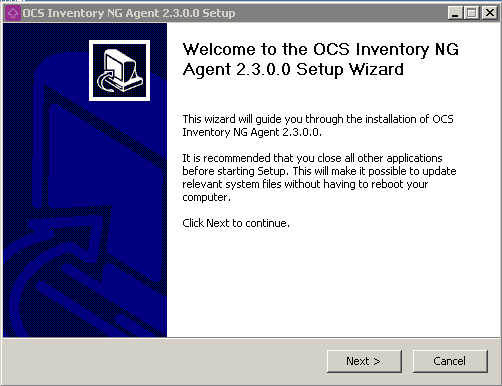
\includegraphics[width=10cm]{imagens/1.PNG}
	\caption{Pressione "\textit{next}" next nessa tela.}
	

\end{figure}

\begin{figure}

	\center
	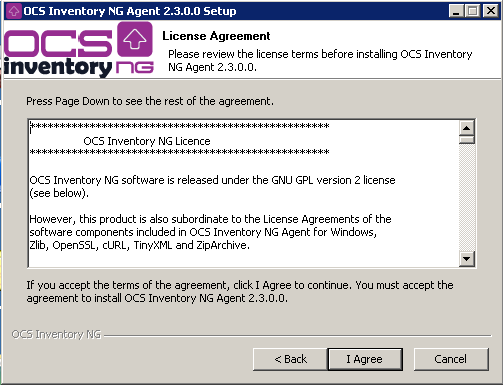
\includegraphics[width=10cm]{imagens/2.PNG}
	\caption{Pressione "\textit{I Agree}" nessa tela.}

\end{figure}

\begin{figure}
	
	\center
	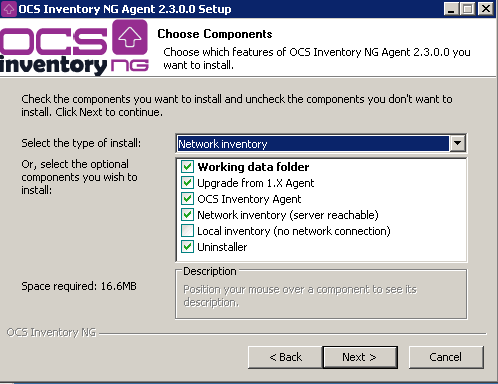
\includegraphics[width=10cm]{imagens/3.PNG}
	\caption{Pressione "\textit{next}" nessa tela.}

\end{figure}

\begin{figure}
	
	\center
	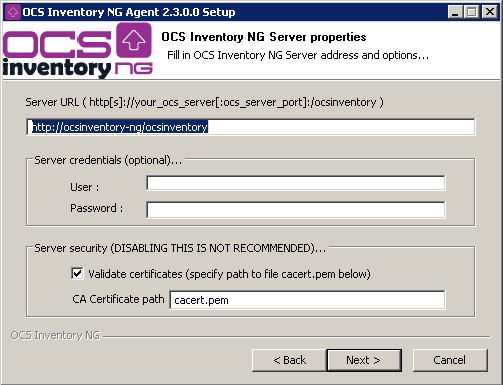
\includegraphics[width=10cm]{imagens/4.PNG}
	\caption{Pressione "\textit{next}" nessa tela.}
	 
\end{figure}

\begin{figure}
	
	\center
	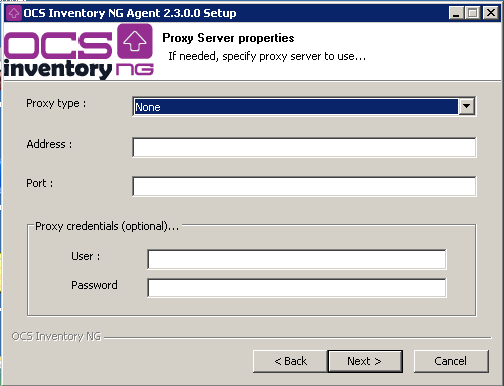
\includegraphics[width=10cm]{imagens/5.PNG}
	\caption{Essa tela deve ser preenchida com as configurações de proxy da sua rede, se houver um.}
	 
\end{figure}

\begin{figure}
	
	\center
	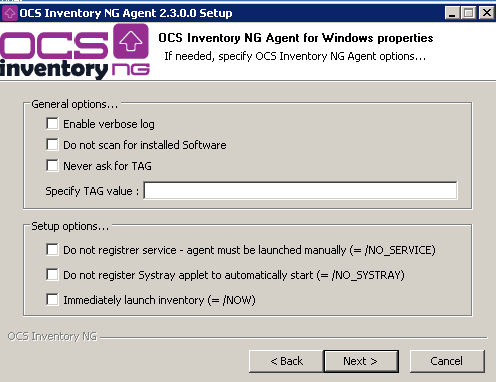
\includegraphics[width=10cm]{imagens/6.PNG}
	\caption{Tela de configuração do agente. Não selecionei nada para esse ambiente.}
	 
\end{figure}

\begin{figure}
	
	\center
	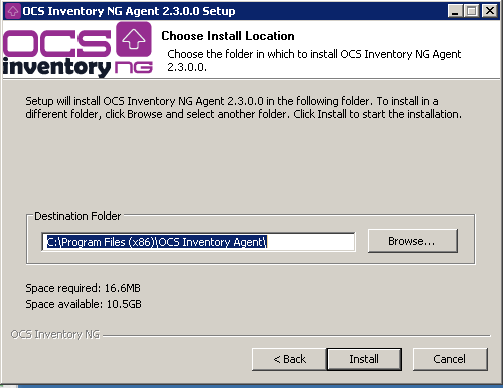
\includegraphics[width=10cm]{imagens/7.PNG}
	\caption{Escolha o local e clique em instalar.}
	 
\end{figure}

\pagebreak

\subsection{Instalação no Linux}

Para instalação no Debian (Jessie) basta digitar o seguinte comando:

\begin{verbatim}
	# apt install ocsinventory-agent
\end{verbatim}

No momento da instalação ele mesmo ira solicitar o IP do servidor, basta informar ao sistema e o resto é automático. O nome do pacote varia pouco de acordo com as distribuições, bastando assim, usar um comando de busca em sua maquina, procurando por OCS, basta encontrar o pacote e fazer a instalação, para o centOS, ficaria assim:

\begin{verbatim}
	# yum search ocs
\end{verbatim}

\subsection{Instalação no MacOSx}

Para instalação no MacOSx faça o \textit{dowload} do arquivo \textit{pkg} neste \href{https://github.com/OCSInventory-NG/UnixAgent/releases/download/2.1.1/Ocsinventory_Agent_MacOSX-2.1.1.pkg.zip}{link} e prossiga normalmente com a instalação.

\subsection{Instalação no Android}

Para instalação no \textit{Android} faça o \textit{dowload} do arquivo \textit{apk} neste \href{https://github.com/OCSInventory-NG/AndroidAgent/releases/download/2.3/OCSNG-Android-Agent-2.3.0.apk}{link} e prossiga normalmente com a instalação.




\end{document}